\section{Aufbau und Durchführung}
\subsection{Aufbau}
Der Aufbau des Versuches ist relativ simpel (\ref{fig:1}) . Auf der einen Seite befindet sich die Strahlungsquelle, in unserem
Fall Cs-137, welches von großes Bleiböcken abgeschirmt, sodass ein schmaler Strahlengang entsteht. Gegenüber 
von der Quelle sitzt ein NaJ-Detektor. Mit diesem wird die $\gamma$-Strahlung detektiert. 

\noindent
Unterhalb des Strahlengangs befindet sich eine Platte, auf welche sich Proben montieren lassen. Diese lässt 
sich verschieben und drehen. Im Versuch wurden auf dieser mehrere Würfel platziert. 2 waren gefüllt mit einem
umbekannten Metall, einer war leer (für eine Referenzmessung) und einer war gefüllt mit 27 kleineren Würfeln
, welche das Volumen des großen Würfels füllen.

\begin{figure}[H]
	\centering
	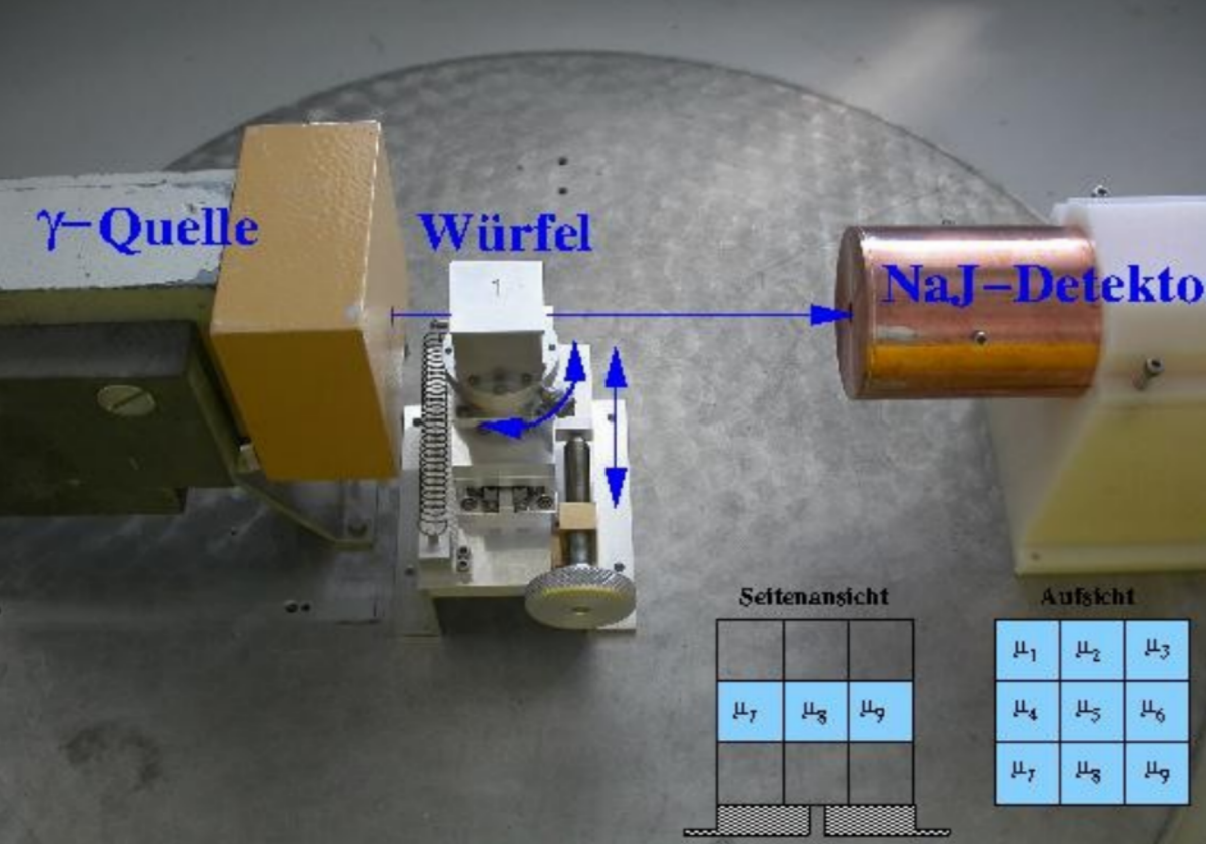
\includegraphics{aufbau.png}
	\caption{Foto vom Aufbau des Experimentes \biber}
	\label{fig:1}
\end{figure}

\subsubsection{Szintillationsdetektor}


\subsubsection{Multichannelanalyzer}



\subsection{Durchführung}



